%--------------------------------------------------------------------%
%
% Berkas utama templat LaTeX.
%
% author Petra Barus, Peb Ruswono Aryan
%
%--------------------------------------------------------------------%
%
% Berkas ini berisi struktur utama dokumen LaTeX yang akan dibuat.
%
%--------------------------------------------------------------------%

\documentclass[12pt, a4paper, onecolumn, oneside, final]{book}

%-------------------------------------------------------------------%
%
% Konfigurasi dokumen LaTeX untuk laporan tesis IF ITB
%
% @author Petra Novandi
%
%-------------------------------------------------------------------%
%
% Berkas asli berasal dari Steven Lolong
%
%-------------------------------------------------------------------%

%
% Ukuran kertas
%
\special{papersize=210mm,297mm}


%
% Used packages
%
\usepackage[top=3cm,bottom=4cm,left=4cm,right=3cm]{geometry} % Setting margin
\usepackage[bahasa]{babel}      % Judul bahasa Indonesia
\usepackage[utf8]{inputenc}     % Encoding
\usepackage[natbibapa]{apacite} % citation: natbib dengan format apacite
\usepackage[dvipsnames]{xcolor} % Using color
\usepackage{mathptmx}
\usepackage{csquotes}
\usepackage{graphicx}
\usepackage{titling}
\usepackage{blindtext}          % Lorem ipsum filling
\usepackage{sectsty}
\usepackage{chngcntr}
\usepackage{etoolbox}
\usepackage{hyperref}           % Package untuk link di daftar isi.
\usepackage{titlesec}           % Package Format judul
\usepackage{parskip}
\usepackage{ragged2e}
\usepackage{times}              % Font yang dipake
\usepackage{booktabs}
\usepackage{longtable}
\usepackage{array}
\usepackage{caption}
\usepackage{enumitem}
\usepackage{listings}
\usepackage{textcase}
\usepackage{setspace}
\usepackage{afterpage}
\usepackage{amsmath,amsfonts}
\usepackage{hyperref}
\usepackage{hypcap}
\usepackage{todonotes}
\usepackage{fancyvrb}
\usepackage{relsize}
\usepackage{tocloft}

%
% Setting ToC
%
% \titleformat{\section}{\large\MakeUppercase}{\thesection}{1em}{}
\renewcommand{\cftbeforetoctitleskip}{0em}
\renewcommand{\cfttoctitlefont}{\hfill\Large\bfseries\MakeUppercase}
\renewcommand{\cftaftertoctitle}{\hfill\hfill}

\renewcommand{\cftbeforeloftitleskip}{0em}
\renewcommand{\cftloftitlefont}{\hfill\Large\bfseries\MakeUppercase}
\renewcommand{\cftafterloftitle}{\hfill}

\renewcommand{\cftbeforelottitleskip}{0em}
\renewcommand{\cftlottitlefont}{\hfill\Large\bfseries\MakeUppercase}
\renewcommand{\cftafterlottitle}{\hfill}

\renewcommand{\cftchappresnum}{BAB\space}
\renewcommand{\cftchapnumwidth}{5em}


% /////////////////////////////////////////////////////////
% \usepackage{appendix}
\newcommand{\listappendixname}{Daftar Lampiran}
\newlistof{appendix}{app}{\listappendixname}
\setcounter{appdepth}{2}

\renewcommand{\theappendix}{\Alph{appendix}}
\renewcommand{\cftappendixpresnum}{Lampiran\space}
\renewcommand{\cftappendixnumwidth}{1in}

\renewcommand{\cftbeforeapptitleskip}{0em}
\renewcommand{\cftapptitlefont}{\hfill\Large\bfseries\MakeUppercase}
\renewcommand{\cftafterapptitle}{\hfill\hfill}

\renewcommand{\appendix}[1]{%
  \refstepcounter{appendix}%
  \chapter{Lampiran\space\theappendix\space #1}%
  \addcontentsline{app}{appendix}{\protect\numberline{\theappendix}#1}%
  % \par
}



%
% Ubah Citation menjadi bahasa Indonesia.
%
\bibliographystyle{apacite}
\renewcommand{\BBAA}{dan}  % between authors in parenthetical cites and ref. list
\renewcommand{\BBAB}{dan}  % between authors in in-text citation
\renewcommand{\BAnd}{dan}  % for ``Ed. \& Trans.'' in ref. list
\renewcommand{\BOthers}{dkk}


\lstdefinestyle{code}{
    belowcaptionskip=\baselineskip,
    breaklines=true,
    frame=L,
    xleftmargin=40pt,
    framexleftmargin=10pt,
    numbersep=20pt,
    numbers=left,
    stepnumber=1,
    language=C,
    basicstyle=\linespread{1.25}\footnotesize\ttfamily,
    keywordstyle=\bfseries\color{green!40!black},
    commentstyle=\itshape\color{purple!40!black},
    stringstyle=\color{orange},
}
\lstMakeShortInline[columns=fixed]|

\lstdefinestyle{algorithm}{
    belowcaptionskip=\baselineskip,
    breaklines=true,
    frame=tblr,
    xleftmargin=25pt,
    framexleftmargin=5pt,
    numbersep=15pt,
    numbers=left,
    stepnumber=1,
    language=pascal,
    basicstyle=\linespread{1.15}\footnotesize\rmfamily,
    keywordstyle=\bfseries\color{green!40!black},
    commentstyle=\itshape\color{purple!40!black},
    stringstyle=\color{orange},
    mathescape=true,
    literate={:=}{$\leftarrow{}$}{1}{beta}{$\beta$}{1},
}

\usepackage[chapter]{algorithm}
\usepackage{algorithmicx}
\usepackage[noend]{algpseudocode}

\makeatletter  % Add this!!!!
 \renewcommand{\ALG@name}{Pseudocode} %doesnt work
\makeatother   % Add this also

% \renewcommand{\thealgorithm}{\arabic{chapter}.\arabic{algorithm}}
% \renewcommand{\algorithmicxname}{Pseudocode}%
\newcommand*\Let[2]{\State #1 $\gets$ #2}
\algrenewcommand\algorithmicrequire{\textbf{Precondition:}}
\algrenewcommand\algorithmicensure{\textbf{Postcondition:}}


%
% Setting include file code/data untuk lampiran
%
% redefine \VerbatimInput
\RecustomVerbatimCommand{\VerbatimInput}{VerbatimInput}{
  fontsize=\relsize{-2},
  baselinestretch=0.75,
  frame=lines,  % top and bottom rule only
  framesep=1.5em, % separation between frame and text
  labelposition=topline,
}

%
% Setting format judul
%
\chapterfont{\centering \Large}
\titleformat{\chapter}[display]
  {\Large\centering\bfseries}
  {\chaptertitlename\ \thechapter}{0pt}
    {\Large\bfseries\uppercase}
\titlespacing*{\chapter}{0pt}{-25pt}{40pt}

\titleformat{\paragraph}
{\normalfont\normalsize\bfseries}{\theparagraph}{1em}{}

\titlespacing*{\paragraph}
{0pt}{3.25ex plus 1ex minus .2ex}{1.5ex plus .2ex}

\titlespacing*{\section} {0pt}{2.5ex plus 1ex minus .2ex}{1.3ex plus .2ex}
\titlespacing*{\subsection} {0pt}{2.25ex plus 1ex minus .2ex}{0.5ex plus .2ex}


%
% Setting nomor pada subbsubbab di body document dan ToC
%
\setcounter{secnumdepth}{3}
\setcounter{tocdepth}{3}

%
% Counter untuk figure dan table.
%
\counterwithin{figure}{chapter}
\counterwithin{table}{chapter}

%
% Line satu setengah spasi
%
\renewcommand{\baselinestretch}{1.5}



\begin{document}

    %-------------------------------------------------------------------------%
    % Set Variable
    %-------------------------------------------------------------------------%
    \newcommand{\thetitle}
      {Paralelisasi Library big integer pada Transport Layer Security (TLS) Handshake}
    \newcommand{\thedatemy}
      {OKTOBER 2019}
    \newcommand{\thedatedmy}
      {8 Oktober 2019}
    \newcommand{\theauthor}
      {Muhammad Reza Ramadhan}
    \newcommand{\thestudentnumber}
      {13514107}


    %-------------------------------------------------------------------------%
    % Front Matter
    %-------------------------------------------------------------------------%
    \frontmatter
    %!TEX root = ../../tugas-akhir.tex
\clearpage
\pagestyle{empty}

\begin{center}
\smallskip

    \large \bfseries \MakeUppercase{\thetitle}
    \vfill

    \large Laporan Tugas Akhir
    \vfill

    \normalsize Disusun sebagai syarat kelulusan tingkat sarjana
    \vfill

    \normalsize Oleh

    \large \theauthor

    \large NIM: \thestudentnumber

    \vfill
    \begin{figure}[h]
        \centering
      	
\includegraphics[width=0.15\textwidth,natwidth=700,natheight=1021]{resources/cover-ganesha.jpg}
    \end{figure}
    \vfill

    \large
    \uppercase{
        Program Studi Teknik Informatika \\
        Sekolah Teknik Elektro dan Informatika \\
        Institut Teknologi Bandung \\
        \thedatemy
    }

\end{center}

\clearpage

    %!TEX root = ../../tugas-akhir.tex
\clearpage
\pagestyle{empty}

\begin{center}
\smallskip

    \large \bfseries \MakeUppercase{\thetitle}
    \vfill

    \large Laporan Tugas Akhir
    \vfill

    \normalsize Oleh

    \large \theauthor

    \large NIM: \thestudentnumber

    \large Program Studi Teknik Informatika

    \normalsize \normalfont Sekolah Teknik Elektro dan Informatika \\
    Institut Teknologi Bandung \\

    \vfill
    \normalsize \normalfont
    Telah disetujui dan disahkan sebagai Laporan Tugas Akhir
    \\[0.1em]
    di Bandung, pada tanggal \thedatedmy.

    \vfill
    \setlength{\tabcolsep}{12pt}
    \begin{tabular}{c@{\hskip 0.5in}c}
        Pembimbing I, & Pembimbing II \\
        & \\
        & \\
        & \\
        & \\
        \underline{Dr. Ir. Rinaldi Munir, MT.} & \underline{Dr. Judhi Santoso M.Sc.} \\
        NIP 196512101994021001 & NIP 196302041989031002 \\
    \end{tabular}

\end{center}
\clearpage

    %!TEX root = ../../tugas-akhir.tex
\chapter*{Lembar Pernyataan}

Dengan ini saya menyatakan bahwa:

\begin{enumerate}

    \item Pengerjaan dan penulisan Laporan Tugas Akhir ini dilakukan tanpa menggunakan bantuan yang tidak dibenarkan.
    \item Segala bentuk kutipan dan acuan terhadap tulisan orang lain yang digunakan di dalam penyusunan laporan tugas akhir ini telah dituliskan dengan baik dan benar.
    \item Laporan Tugas Akhir ini belum pernah diajukan pada program pendidikan di perguruan tinggi mana pun.

\end{enumerate}

Jika terbukti melanggar hal-hal di atas, saya bersedia dikenakan sanksi sesuai dengan Peraturan Akademik dan Kemahasiswaan Institut Teknologi Bandung bagian Penegakan Norma Akademik dan Kemahasiswaan khususnya Pasal 2.1 dan Pasal 2.2.
\vspace{15mm}

Bandung, \thedatedmy
\vspace{25mm}

\underline{\theauthor}\\
NIM \thestudentnumber


    \pagestyle{plain}

    %!TEX root = ../../tugas-akhir.tex
\clearpage
\chapter*{Abstrak}
\addcontentsline{toc}{chapter}{ABSTRAK}

\begin{center}
  \large \bfseries \MakeUppercase{\thetitle}

  \normalsize \normalfont Oleh

  \theauthor

  NIM : \thestudentnumber
\end{center}


%taruh abstrak bahasa indonesia di sini
\begin{singlespacing}
% \setstretch{1.0}

\Blindtext

\end{singlespacing}


Kata Kunci: \textit{Big Integer, Transport Layer Security}, Algoritma Karatsuba

    % \clearpage
\chapter*{Abstract}
\addcontentsline{toc}{chapter}{Abstract}

%put your abstract here
% \blindtext

\clearpage
    \chapter*{Kata Pengantar}
\addcontentsline{toc}{chapter}{KATA PENGANTAR}

\Blindtext

\begin{flushright}
Bandung, \thedatedmy
\\[2cm]

\theauthor
\end{flushright}


    %-------------------------------------------------------------------------%
    % Daftar Isi, Tabel & Gambar
    %-------------------------------------------------------------------------%
    % \clearpage
    \addcontentsline{toc}{chapter}{DAFTAR ISI}
    {\tableofcontents}



    % \clearpage
    % {
    %     \let\oldnumberline\numberline
    %     \renewcommand{\numberline}{\figurename~\oldnumberline}
    %     \listofappendix
    % }
    \addcontentsline{toc}{chapter}{DAFTAR LAMPIRAN}

    % \clearpage
    {
        \let\oldnumberline\numberline
        \renewcommand{\numberline}{\figurename~\oldnumberline}
        \listoffigures
    }

    \addcontentsline{toc}{chapter}{DAFTAR GAMBAR}

    % \clearpage
    {
        \let\oldnumberline\numberline
        \renewcommand{\numberline}{\tablename~\oldnumberline}
        \listoftables
    }

    \addcontentsline{toc}{chapter}{DAFTAR TABEL}

    %-------------------------------------------------------------------------%
    % Konfigurasi Numbering di Bab
    %-------------------------------------------------------------------------%
    \renewcommand{\chaptername}{BAB}
    \renewcommand{\thechapter}{\Roman{chapter}}

    \mainmatter


    % -------------------------------------------------------------------------%
    % Daftar BAB
    % -------------------------------------------------------------------------%
    \chapter{Pendahuluan}


\section{Latar Belakang}

% basically overview TLS, apa itu TLS
\textit{Transport Layer Security} (TLS) merupakan sebuah protokol yang berguna untuk menjamin keamanan dan kerahasiaan dari sebuah pesan yang dikirim melalui jaringan. Saat ini, TLS umum digunakan sebagai sebuah \textit{security layer} dari berbagai protokol yang saat ini umum digunakan di Internet seperti \textit{Hyper-Text Transfer Protocol}, (HTTP) \textit{File Transfer Protocol} (FTP), ataupun \textit{Simple Mail Transfer Protocol} (SMTP). Penggunaan TLS sebagai \textit{layer} tambahan membuat TLS dapat digunakan untuk berbagai protokol dimana keamanan informasi merupakan hal yang penting.

% Apa itu TLS Handshake, masalah TLS handshake sekarang
Sebuah koneksi TLS akan didahului dengan adanya TLS \textit{handshake} untuk menentukan \textit{symmetric key} dan \textit{cipher} yang akan digunakan oleh \textit{client} dan \textit{server} untuk berkomunikasi setelahnya. Sayangnya, waktu yang digunakan untuk TLS \textit{handshake} masih cukup signifikan; penggunaan TLS pada HTTP dapat meningkatkan waktu \textit{load} pada sebuah \textit{website} menjadi 1,2 hingga 3 kali lebih lambat dibandingkan dengan \textit{website} yang tidak menggunakan TLS \citep{cost_of_s}. Hal ini merupakan salah satu alasan kenapa saat ini TLS belum digunakan oleh seluruh layanan yang ada di internet.

% Show bagian mana dari TLS yang bikin lambat, kenalin ke big integer
Penggunaan alogritma kriptografi kunci publik pada dalam TLS Handshake membutuhkan waktu komputasi yang relatif lebih besar dibandingkan dengan proses lain. Waktu yang digunakan oleh komputasi kriptografi kunci publik sendiri adalah 13-59\% dari seluruh proses komputasi pada TLS \citep{perf_tls}. Komputasi kriptografi kunci publik perlu menggunakan bilangan bulat yang besar untuk memastikan kunci yang digunakan dalam kriptografi aman. Komputasi bilangan bulat besar (\textit{big integer}) tersebutlah yang menyebabkan komputasi kriptografi kunci publik  memerlukan waktu yang lama.

% Metode yang disarankan untuk meningkatkan TLS handshake
% Ini perlu nyantumin paper engga?
Terdapat beberapa metode yang telah disarankan untuk meningkatkan kinerja TLS \textit{handshake} seperti melakukan optimisasi pada algoritma Rivest–Shamir–Adleman (RSA) dengan pemrograman paralel, melakukan \textit{batching} pada proses RSA di server, ataupun melakukan \textit{rebalancing} sehingga komputasi pada client lebih sulit daripada server. Solusi lain yang dapat digunakan adalah memparalelkan komputasi \textit{big integer} sehingga komputasi tersebut dapat dilakukan dalam waktu lebih pendek.

% Solusi big integer, berbagai algoritma yang ada dan kemungkinannya untuk diparalelkan
% Montgomery italic ga? nama orang
Komputasi big integer bukanlah hal yang baru dalam dunia ilmu komputer. \citet{modern_comp_math} memberikan tujuh algoritma yang dapat digunakan dalam perkalian, delapan algoritma pembagian, serta berbagai alternatif algoritma  yang dapat digunakan dalam setiap operasi dalam komputasi big integer. Terdapat beberapa juga beberapa algoritma yang dapat dijalankan secara paralel, seperti metode representasi \textit{Residue Number Systems} dan algoritma Montgomery pada komputasi perkalian modular.

Terdapat dua pilihan yang dapat digunakan untuk menjalakan komputasi \textit{big integer} secara paralel, yaitu menjalakan komputasi pada CPU atau GPU. Penggunaan GPU dalam memparalelkan komputasi kriptografi kunci publik dapat menghasilkan jumlah \textit{transaction per second} hingga 45 kali lebih besar dibandingkan dengan penggunaannya pada CPU \citep{gpu_vs_cpu}. Namun, GPU tidak umum digunakan pada data center sehingga penggunaan GPU dalam komputasi kriptografi kunci publik pada kehidupan sehari-hari tidak realistis. Dengan umumnya \textit{multicore} CPU yang digunakan server, penggunaan CPU dalam paralelisasi lebih realistis.


\section{Rumusan Masalah}

Sesuai dengan pembahasan yang ada pada latar belakang, diketahui bahwa penggunaan pemrograman paralel dalam komputasi \textit{big integer} merupakan salah satu metode yang dapat digunakan untuk meningkatkan kinerja TLS \textit{Handshake}. Maka dari itu, tugas akhir ini akan fokus pada pengembangan algoritma paralel yang digunakan dalam komputasi \textit{big integer} dan implementasinya pada TLS \textit{handshake}. Dalam pengembangannya, terdapat berapa masalah yang akan menjadi perhatian utama dalam tugas akhir ini, yaitu:

\begin{enumerate}
  \item Algoritma paralel seperti apa yang akan diimplementasikan dalam komputasi \textit{big integer}?
  \item Bagaimana cara mengintegrasikan algoritma paralel tersebut ke dalam library \textit{big integer}?
  \item Apakah penggunaan algoritma paralel dalam komputasi \textit{big integer} dapat meningkatkan kinerja dari TLS \textit{handshake}?
\end{enumerate}

\section{Tujuan}

Dalam penyelesaian tugas akhir ini terdapat beberapa tujuan yang akan dicapai, yaitu:
\begin{enumerate}
  \item Menemukan algoritma paralel yang dapat digunakan dalam komputasi \textit{big integer}.
  \item Mengintegrasikan algoritma tersebut dalam sebuah implementasi library \textit{big integer}.
  \item Mengukur peningkatan kinerja dari TLS \textit{handshake} setelah mengimplementasikan algoritma paralel RSA.
\end{enumerate}

\section{Batasan Masalah}

Tugas akhir ini akan membahas mengenai optimisasi algoritma RSA pada sebuah implementasi TLS \textit{handshake}. Adapun batasan masalah yang terdapat pada tugas akhir ini adalah:

\begin{enumerate}
  \item Paralelisasi library big integer tidak memperhatikan masalah keamanan pada sistem yang menggunakannya.
  \item Implementasi TLS memanfaatkan perangkat lunak opensource OpenSSL versi 1.1.1.
  \item Ciphersuite yang digunakan dalam penelitian ini adalah TLS\_DH\_RSA\_WITH\_AES\_256\_CBC\_SHA256.
  \item CPU yang digunakan pada implementasi ini adalah Intel 64-bit yang minimal memiliki enam belas \textit{core}.
\end{enumerate}

\section{Metodologi}

Pengerjaan tugas akhir ini akan melalui beberapa tahap, yaitu:
\begin{enumerate}
  \item Analisis Masalah

  Tugas akhir akan dimulai dengan dilakukannya analisis mengenai masalah terhadap implementasi TLS \textit{handshake} yang ada pada saat ini. Pada tahap ini akan dipelajari juga mengenai solusi-solusi untuk meningkatkan kinerja dari TLS \textit{handshake} yang sudah tersedia pada saat ini. Dari solusi yang sudah ada tersebut, penulis akan mencari penyebab solusi itu belum diimplementasikan pada TLS \textit{handshake} dan mencari solusi baru yang mungkin untuk diimplementasikan.

  \item Perancangan Solusi dan Pengujian

  Perancangan solusi dibuat sebagai kerangka dasar atas solusi dari masalah yang telah ditemukan pada langkah sebelumnya. Pada tahap ini akan dirancang arsitektur solusi beserta cara untuk menerapkannya pada TLS handshake yang sudah ada. Selain itu, akan dibuat juga rencana pengujian terhadap implementasi solusi. Rencana pengujian akan dibuat sehingga percobaan dilakukan dalam batas masalah yang ada dan dapat dilakukan sesuai metode sains.

  \item Implementasi Solusi

  Pada tahap ini, penulis akan mengimplementasikan rancangan solusi yang sudah dibuat dalam sebuah bentuk perangkat lunak yang dapat digunakan dalam dunia sehari-hari. Hasil implementasi yang dibuat tentu ditujukan untuk menyelesaikan masalah yang ada.

  \item Pengujian dan Evaluasi

  Pengujian akan dilakukan berdasarkan rancangan pengujian telah ada. Pengujian dilakukan untuk mengetahui apakah solusi yang diberikan merupakan solusi terbaik dari masalah yang ada. Hasil dari pengujian akan digunakan sebagai data evaluasi dan penarikan kesimpulan.

\end{enumerate}


\section{Sistematika Laporan}
\todo[inline]{Diisi nanti kalo laporan udah beres}

% \blindtext
% Penulisan tugas akhir ini akan terdiri dari lima bab yaitu: BAB I Pendahuluan, BAB II Studi Literatur, BAB III Analisis Solusi, BAB IV Rancangan, Implementasi dan Pengujian, BAB V Penutup.
%
% Bab satu memaparkan mengenai latar belakang pembuatan tugas akhir ini, masalah utama yang dibahas, tujuan pembuatan tugas akhir, serta metodologi yang akan dilakukan selama pembuatan tugas akhir. Bab ini dibuat sebagai pendahuluan dan akan mencakup ringkasan dari sebagian besar hal yang dibahas pada tugas akhir.
%
% Bab dua akan membahas mengenai teori dasar yang sudah ada mengenai protokol TLS, algoritma RSA, serta pengembangan dari algoritma RSA melalui pemrograman paralel yang sudah ada. Teori yang diambil akan bersumber dari literatur terpercaya serta dokumentasi resmi dari protokol TLS.
%
% Bab tiga menggambarkan solusi yang digunakan untuk menyelesaikan masalah yang ada, kenapa digunakan solusi tersebut, serta hipotesa peningkatan kinerja dari TLS handshake setelah solusi yang dibuat diimplementasikan.
%
% Bab empat memperlihatkan rancangan implementasi dari solusi, proses implementasi solusi tersebut, serta hasil pengujian dari implementasi tersebut pada kinerja TLS handshake.
%
% Bab lima mendeskripsikan hasil kesimpulan dari solusi yang dibuat untuk menyelesaikan masalah serta saran yang dapat dilakukan untuk pengembangan dan perbaikan agar implementasi ini dapat menghasilkan hasil yang lebih baik.

    %!TEX root = ../../tugas-akhir.tex
\chapter{STUDI LITERATUR}

% Outline:
% 2.1 big integer
% 2.2 Kripto
% 2.3 TLS
% 2.4 Parallel Programming
% 2.5 Other maths Chinese remainder theorem, modulo math, etc
% 2.6 Relevant Researches

%!TEX root = ../../../tugas-akhir.tex
\section{Kriptografi}
  Kriptografi adalah sebuah ilmu yang mempelajari cara pengiriman pesan sehingga tidak memungkinkan bagi pihak ketiga untuk membaca ataupun memanipulasi isi pesan tersebut. Kriptografi sudah digunakan sejak jaman kerajaan Romawi Kuno dengan digunakannya Caesar Cipher oleh Julius Caesar untuk berkomunikasi dengan Jendral Perangnya. Kriptografi modern berfokus pada teori matematis dan kesulitan pihak ketiga dalam membaca atau memanipulasi pesan secara komputasional.

  Pada berbagai literatur kriptografi sering dikenal beberapa istilah seperti:
  \begin{enumerate}[label=\roman*.]
    \item \textit{sender}, yaitu pihak pengirim pesan
    \item \textit{receiver}, yaitu pihak penerima pesan
    \item \textit{eavesdropper}, yaitu pihak ketiga yang berusaha membaca atau memodifikasi pesan yang dikirim
    \item \textit{plaintext}, yaitu pesan yang dikirim. \textit{Plaintext} tidak harus merupakan sebuah teks namun dapat berupa audio, gambar, ataupun file binary.
    \item \textit{ciphertext}, yaitu pesan yang telah diubah oleh algoritma tertentu
    \item enkripsi, yaitu proses pengubahan \textit{plaintext} menjadi \textit{ciphertext}
    \item dekripsi, yaitu proses pengubahan \textit{ciphertext} menjadi \textit{plaintext}
    \item \textit{key}, yaitu nilai yang digunakan dalam enkripsi ataupun dekripsi
  \end{enumerate}

  Pada umumnya, proses yang terjadi dalam penggunaan kriptografi pada sebuah pengiriman sebuah data dapat dilihat pada Gambar ~\ref{fig:krypto_system}:

  \begin{figure}[h]
    \centering
    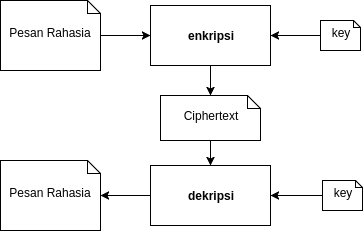
\includegraphics[width=0.6\textwidth]{resources/ch-2/crypto-system.jpg}
    \caption{Sistem pengiriman data menggunakan kriptografi}
    \label{fig:krypto_system}
  \end{figure}

  Terdapat dua macam tipe kriptografi yang saat ini umum digunakan. Kriptografi kunci simetri adalah sebuah sistem kriptografi dimana proses enkripsi dan dekripsi menggunakan kunci yang sama. Kriptografi asimetris atau biasa disebut kriptografi kunci publik merupakan sebuah sistem kriptografi dimana proses enkripsi dan dekripsi menggunakan dua kunci yang berbeda.

  Masalah utama yang dihadapi pada sistem kriptografi kunci simetri adalah bagaimana dua pihak dapat menentukan sebuah kunci yang akan digunakan tanpa sepengetahuan pihak ketiga. Pada algoritma kriptografi modern, terdapat beberapa metode untuk mengirimkan kunci simetri pada pihak lain, diantaranya adalah mendekripsi key tersebut dengan algoritma kriptografi kunci publik atau dengan menggunakan algoritma \textit{key exchange}.

  \subsection{Kriptografi Kunci Publik}

    Kriptografi kunci publik adalah sebuah sistem kriptografi dimana proses enkripsi dan dekripsi dilakukan dengan kunci yang berbeda. Umumnya terdapat dua macam kunci yang terdapat pada sistem ini, yaitu \textit{public key} yang dapat dipublikasikan kepada siapapun dan \textit{private key} yang hanya dimiliki oleh pemilik kunci tersebut. \textit{Public key} digunakan untuk mengenkripsi data, sementara \textit{private key} digunakan oleh pemilik kunci untuk mendekripsi data tersebut.

    Salah satu kebutuhan utama yang terdapat pada kriptografi kunci publik adalah sebuah algoritma yang mudah untuk dikomputasi dalam satu arah, namun sulit untuk dilakukan sebaliknya. Algoritma yang digunakan umumnya berdasar pada masalah matematis seperti faktorisasi bilangan bulat, logaritma diskrit, atau hubungan kurva eliptik. Sebagai contoh, jika kita memiliki dua bilangan bulat maka dapat dengan mudah mengkalikan dua bilangan tesebut dan mendapat satu bilangan bulat baru; namun kita tidak bisa dengan mudah menentukan dua bilangan bulat yang merupakan faktor dari sebuah bilangan bulat.

    Saat ini komputasi kriptografi kunci publik masih memerlukan proses komputasi yang lebih tinggi dibandingkan dengan kriptografi kunci simetris. Maka dari itu, kriptografi kunci publik biasanya hanya dilakukan untuk mengenkripsikan kunci yang akan digunakan dalam kriptografi kunci simetris.

    \subsubsection{Rivest–Shamir–Adleman (RSA)} \label{sec:rsa_theory}
    \todo{edit lagi, bahasanya ngaco}
    RSA merupakan salah satu algoritma kriptografi kunci publik yang hingga saat ini banyak digunakan. Algoritma RSA pertama kali dicetuskan oleh Ron Rivest, Adi Shamir, dan Leonard Adleman pada tahun 1978. RSA berdasar pada sifat matematis bahwa dalam sebuah pemangkatan modular dengan persamaan:
    \begin{equation}
      (m^e)^d  \equiv  m \pmod{n}
    \end{equation}

    Pencarian tiga bilangan bulat n, e, dan d dapat dilakukan dengan mudah; bahkan untuk bilangan n, e, dan d yang sangat besar. Namun, pencarian bilangan d akan susah dilakukan, bahkan jika kita mengetahui bilangan-bilangan lainnya. Selain itu mengingat operasi perpangkatan dapat ditukar, maka proses enkripsi dan dekripsi dapat dilakukan dengan metode yang sama, hanya menggunakan bilangan yang berbeda.

    Terdapat beberapa proses yang terjadi pada algoritma RSA yaitu pembuatan \textit{public} dan \textit{private key}, distribusi \textit{public key}, enkripsi, serta dekripsi. Proses pembuatan public dan private key sendiri dilakukan dalam beberapa tahap yaitu:

    \begin{enumerate}
      \item Pilih dua bilangan prima yang besar, $p$ dan $q$.
      \item Hitung $n = p*q$ dan $ \phi = (p-1)*(q-1)$ .
      \item Pilih sebuah bilangan bulat random $e$ dengan $ 1 < e < \phi$ dan .
      \item Hitung bilangan bulat $d$, dengan $ e*d  \equiv  1 \pmod{\phi} $
    \end{enumerate}

    Dari perhitungan diatas, didapat \textit{public key} $(e, n)$ dan private key $(d, n)$.
    Proses enkripsi pada sebuah data \textit{D} dapat dilakukan melalui beberapa langkah sebagai berikut:
    \begin{enumerate}
      \item Ubah \textit{D} menjadi satu atau beberapa bilangan bulat \textit{m}, dengan \textit{m} berada dalam interval [1..n-1]
      \item Hitung ciphertext \textit{c} untuk masing-masing \textit{m}, dengan $c = m^e \mod n $
    \end{enumerate}

    Sementara itu, proses dekripsi dapat dilakukan dengan menghitung plaintext $m$ dari ciphertext $c$ yang didapatkan dengan $m = c^d \mod n$.


  \subsection{Algoritma Pertukaran Kunci}
  Algoritma pertukaran kunci adalah algoritma yang digunakan untuk menghasilkan sebuah kunci rahasia antara dua atau lebih pihak tanpa diketahui oleh pihak lain \citep{applied_crypto}. Kunci yang dihasilkan dari algortima ini akan digunakan sebagai kunci pada sistem kriptografi simetris.

    \subsubsection{Diffie-Hellman}
    Algoritma Diffie-Hellman (DH) merupakan salah satu algoritma paling awal yang memperkenalkan konsep pertukaran kunci. Walaupun DH merupakan algoritma awal yang ada, DH masih umum digunakan pada sistem kriptografi modern. Kriptografi modern hanya menggunakan modifikasi dari algoritma DH, misalnya dengan menggunakan kurva eliptik sebagai basis perhitungannnya.

    Seperti RSA, DH memiliki basis perpangkatan modulo bilangan bulat. Pada awal algortima DH, dipilih dua nilai publik $p$ dan $g$, dengan $p$ merupakan bilangan prima besar dan $g$ adalah akar primitif modulo dari $p$. Setelah itu, masing-masing pihak akan memilih nilai random $x$ dengan $1 \leq x \leq p-1 $. Setelah nilai random dipilih akan dihitung nilai $pk = g^x \mod p$ pada masing-masing pihak, kemudian nilai $pk$ akan dikirim melalui jaringan pada pihak yang lain. Setelah nilai dari pihak lain diterima, akan dihitung nilai $key = prekey^x \mod p$. Ilustrasi pertukaran kunci dapat dilihat pada Gambar \ref{fig:dh_exchange}.

    \begin{figure}[h]
      \centering
      \includegraphics[width=0.9\textwidth]{resources/ch-2/dh-exchange}
      \caption{Proses pertukaran kunci Diffie-Hellman}
      \label{fig:dh_exchange}
    \end{figure}

    Meskipun nilai $p, g, $ serta $pk$ merupakan nilai publik yang dapat diketahui semua orang, pihak ketiga tidak dapat menghitung nilai akhir $key$ yang didapatkan dari perhitungan pada masing-masing server. Untuk mendapatkan $key$ yang digunakan oleh dua pihak, dibutuhkan nilai random $x$ yang dipilih oleh masing-masing pihak tersebut. Perhitungan nilai $x$ dari nilai $g^x mod p$ merupakan masalah logartima diskrit, yaitu masalah yang sama dengan pencarian kunci privat dari RSA.

%!TEX root = ../../../tugas-akhir.tex
\section{\textit{Transport Layer Security} (TLS)}
  \textit{Transport Layer Security} (TLS) adalah sebuah protokol kriptografi yang menjamin kerahasiaan serta integritas dalam data yang dikirim dalam sebuah koneksi yang tidak dipercaya. TLS pertama kali dikembangkan sebagai \textit{Secure Socket Layer} (SSL) oleh Netscape pada tahun 1995, dan kemudian diresmikan oleh Internet Engineering Task Force (IETF) dalam RFC 2246 pada tahun 1998. SSL dirancang dengan empat tujuan utama yaitu keamanan secara kriptografis, interoperabilitas, kemampuan penambahan protokol, serta efisiensi \citep{perf_tls}.

  TLS dirancang sebagai sebuah protokol perantara antara protokol aplikasi (HTTP, FTP, SMTP) dan protokol transport (TCP, UDP). Semua data yang dikirimkan oleh aplikasi akan dienkripsi terlebih dahulu oleh TLS sehingga data dapat dikirimkan secara terenkripsi. Hal ini dapat mempermudah penggunaan TLS diatas protokol aplikasi mengingat aplikasi hanya perlu mengirimkan data melalui TLS socket alih-alih melalui TCP/UDP socket untuk kemudian dienkripsi dan dikirimkan pada tujuan melalui TCP/UDP socket. Ilustrasi perbandingan antara pengiriman dengan menggunakan TLS dan tidak menggunakan TLS dapat dilihat pada Gambar ~\ref{fig:tls-usage}

  \begin{figure}[h]
    \centering
    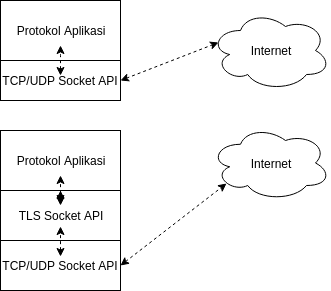
\includegraphics[width=0.6\textwidth]{resources/img/ch-2/tls-usage.png}
    \caption{Perbandingan Penggunaan Protokol TLS pada Aplikasi \protect\citep{perf_tls}}
    \label{fig:tls-usage}
  \end{figure}

  Dewasa ini, TLS umum digunakan sebagai layer keamanan pada protokol aplikasi yang umum digunakan di internet. Berbagai protokol yang awalnya tidak memiliki standar keamanan dapat menggunakan TLS untuk mengamankan aliran data. Sebagai contoh, penggunaan HTTPS dapat memastikan bahwa data-data penting seperti \textit{password}, nomor kartu kredit, ataupun alamat tidak dapat dilihat oleh siapapun kecuali pengguna dan pemilik dari sebuah website.

  TLS merupakan sebuah protokol asimetrik dimana pihak yang melakukan koneksi dapat dibagi menjadi client dan server. TLS menyediakan metode otentikasi sehingga sebuah pihak dapat yakin bahwa ia memang berkomunikasi dengan pihak yang ia inginkan. TLS menyediakan metode otentikasi baik untuk client maupun server, walaupun pada praktiknya biasanya hanya server yang diotentikasi oleh client. Salah satu metode lain adalah TLS memastikan bahwa pesan yang dikirim tidak diubah pada perjalanan dengan adanya penambahan \textit{Message Authentication Code} (MAC) pada semua data yang dikirim.

  Protokol TLS pada dasarnya tersusun dari dua protokol utama, yaitu Protokol TLS \textit{Record} dan Protokol TLS \textit{Handshake}. Protokol TLS Record digunakan untuk mengenkapsulasi data yang diterima oleh protokol aplikasi, sementara itu Protokol TLS Handshake digunakan untuk mengotentikasi client dan server serta melakukan negosiasi mengenai pemilihan penggunaan algoritma enkripsi, kunci yang digunakan, serta pemilihan penggunaan algoritma MAC (Message Authentication Code).

% Pengembang dari TLS sadar bahwa komputasi kriptografis yang digunakan dalam otentikasi server memerlukan biaya komputasi yang cukup tinggi. Karena itulah, TLS memiliki sebuah mekanisme session yang memungkinkan client yang telah menyelesaikan TLS \textit{Handshake} sebelumnya untuk melakukan TLS Handshake secara cepat dengan menggunakan ulang data session yang masih tersimpan pada client. Pada sebuah session, data yang tersimpan diantaranya:
% \begin{description}
%   \item[-] \textit{Session identifier}
%   \item[-] \textit{Peer cerficate}
%   \item[-] \textit{Compression method}
%   \item[-] \textit{Cipher spec}, yaitu pasangan algoritma yang digunakan dalam enkripsi dan MAC.
%   \item[-] \textit{Master secret}, yaitu key 48-byte yang digunakan dalam enkripsi dan dekripsi.
%   \item[-] \textit{is resumable}, menandakan apakah session ini dapat digunakan untuk membuat session baru.
% \end{description}


  \subsection{Protokol TLS \textit{Handshake}}
    TLS \textit{Handshake} adalah protokol yang digunakan untuk melakukan otentikasi serta negosiasi untuk menentukan parameter yang digunakan pada sebuah koneksi TLS. Sebuah TLS \textit{handshake} juga digunakan untuk membuat dan menentukan \textit{session} dari sebuah koneksi TLS. Protokol ini juga mendeskripsikan cara yang digunakan oleh TLS untuk memberikan tanda pada satu sama lain jika terjadi error pada salah satu tahap yang terjadi.

    Tahap yang terjadi dalam sebuah TLS \textit{Handshake} dapat dideskripsikan sebagai berikut:
  \begin{enumerate}
    \item Pengiriman ‘Hello’ sebagai tanda mulainya koneksi.
    \item Pengiriman algoritma yang didukung, nilai random, serta pengecekan untuk penggunaan kembali session.
    \item Pengiriman parameter yang digunakan untuk melakukan komputasi kunci simetris.
    Pengiriman sertifikat oleh server dan otentikasi server oleh client.
    \item Melakukan komputasi kunci simetris secara independen, kemudian menyimpan parameter-parameter yang dibutuhkan untuk penyimpanan data.
    \item Melakukan verifikasi bahwa semua pihak telah menghitung kunci simetris yang sama dan memastikan proses handshake tidak diganggu oleh siapapun.
  \end{enumerate}

    Apabila terdapat \textit{error} pada salah satu tahap diatas, maka akan dikirimkan tanda \textit{error} dan pembuatan koneksi dihentikan seketika. Proses pengiriman data yang terjadi pada sebuah TLS Handshake dapat dilihat pada Gambar ~\ref{fig:tls-handshake}.

    \begin{figure}[h]
      \centering
      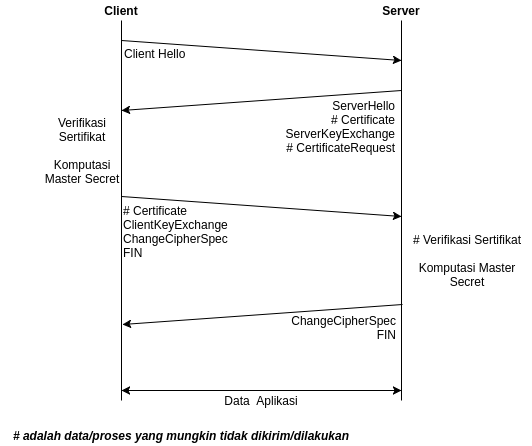
\includegraphics[width=0.6\textwidth]{resources/img/ch-2/handshake.png}
      \caption{Proses Pengiriman Data pada TLS Handshake \protect\citep{rfc5246}}
      \label{fig:tls-handshake}
    \end{figure}

    Pada Gambar ~\ref{fig:tls-handshake}, terlihat bahwa proses handshake merupakan proses yang memakan waktu cukup signifikan. Hal ini disebabkan karena terdapat setidaknya empat kali pengiriman data antara client dan server, selain itu proses \textit{key exchange} dan verifikasi sertifikat yang dilakukan tidak memakan waktu yang singkat.

    Untuk mengatasi hal ini, TLS menyediakan proses handshake singkat dimana client akan menggunakan \textit{session\_id} yang dimilikinya untuk melanjutkan session tersebut. Pada proses ini, client akan mengirimkan data \textit{session\_id} bersama ClientHello; server kemudian akan mencari data session pada session cache dan melanjutkannya jika ditemukan. Jika proses ini gagal, maka proses handshake akan dilakukan seperti biasa. Proses pengiriman data yang dilakukan pada handshake singkat dapat dilihat pada Gambar ~\ref{fig:tls-fast-handshake}.

    \begin{figure}[h]
      \centering
      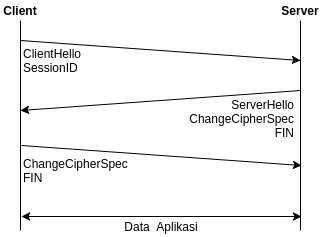
\includegraphics[width=0.6\textwidth]{resources/img/ch-2/fast-handshake.png}
      \caption{Proses Pengiriman Data pada TLS Handshake Singkat \protect\citep{rfc5246}}
      \label{fig:tls-fast-handshake}
    \end{figure}

    Terlihat bahwa penggunaan ulang \textit{session} dapat mempersingkat waktu yang digunakan dalam TLS \textit{handshake} secara signifikan mengingat tidak diperlukannya lagi validasi sertifikat ataupun proses \textit{key exchange}.

  \subsection{Protokol TLS \textit{Record}}
    Protokol TLS \textit{Record} merupakan protokol pemrosesan data yang didapat dari aplikasi untuk kemudian dikirim melalui jaringan dan juga sebaliknya. Ketika TLS menerima data dari sebuah aplikasi, data tersebut akan dibagi menjadi beberapa blok data untuk mempermudah pengolahan, data kemudian akan di-\textit{compress}, ditambahkan MAC, dienkripsi, lalu kemudian dikirim melalui jaringan. Sebaliknya, ketika TLS menerima data dari jaringan, data akan didekripsi, diverifikasi dengan MAC, di-decompress, disusun ulang, lalu dikirim pada aplikasi.

    Pada pengiriman data, TLS menggunakan format data tertentu seperti diilustrasikan pada Gambar ~\ref{fig:tls-record}:
    \begin{figure}[h]
      \centering
      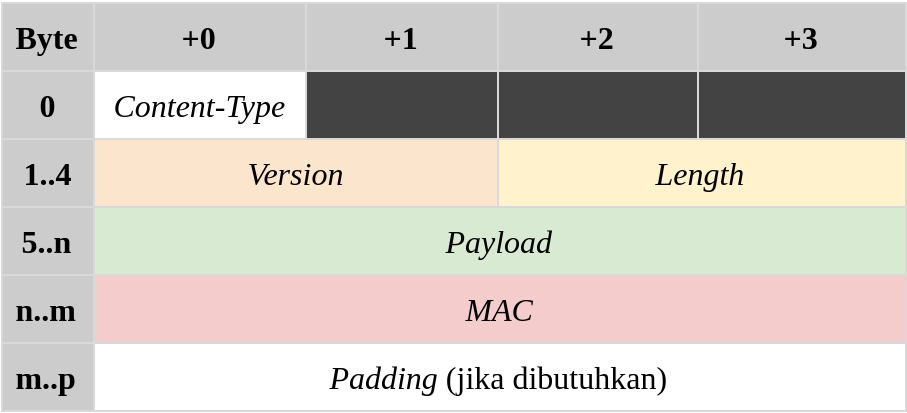
\includegraphics[width=0.6\textwidth]{resources/img/ch-2/tls-record.png}
      \caption{Struktur Sebuah Record TLS \protect\citep{rfc5246}}
      \label{fig:tls-record}
    \end{figure}

    % Untuk setiap koneksi yang ada, TLS akan beberapa nilai yang menggambarkan status dari koneksi tersebut. Salah satu data yang disimpan adalah algoritma kompresi, enkripsi, serta MAC yang digunakan. Selain itu, berbagai parameter yang diperlukan oleh setiap algoritma seperti kunci yang digunakan untuk enkripsi dan MAC juga akan disimpan.

    Proses enkripsi yang terjadi pada tahap ini akan menggunakan sebuah algoritma kriptografi kunci simetris seperti AES ataupun RC4 dengan kunci yang digunakan dalam algoritma tersebut didapatkan oleh client dan server pada TLS Handshake. Penggunaan kriptografi kunci simetris akan membuat proses enkripsi dan dekripsi menjadi relatif lebih cepat jika dibandingkan dengan penggunaan algoritma kriptografi kunci publik.


  \subsection{Ciphersuite}
    \textit{Ciphersuite} adalah sebuah kumpulan dari algoritma yang digunakan dalam TLS \textit{handshake}. Sebuah \textit{ciphersuite} akan terdiri dari algoritma tertentu yang digunakan dalam sebuah koneksi TLS. Kumpulan algoritma tersebut biasanya akan berisi algoritma otentikasi, algoritma \textit{key exchange}, algoritma enkripsi data pada TLS record, serta algoritma MAC. Terdapat banyak kombinasi dari ciphersuite yang umum digunakan pada protokol TLS, beberapa diantaranya memiliki tingkat keamanan yang lebih rendah dibandingkan dengan ciphersuite lain.

    Setiap TLS \textit{client} dan \textit{server} akan memiliki daftar \textit{ciphersuite} yang didukung. Daftar tersebut akan mengurutkan setiap ciphersuite dengan urutan tertentu berdasarkan preferensi dari masing-masing client dan server. Urutan ini biasanya disusun berdasarkan tingkat keamanan dari masing-masing \textit{ciphersuite}. \textit{Ciphersuite} yang memiliki tingkat keamanan tinggi akan memiliki urutan yang lebih prioritas dibandingkan \textit{ciphersuite} dengan tingkat keamanan yang lebih rendah.

    Sebuah ciphersuite biasanya memiliki format penulisan tertentu, sebagai contoh TLS\_DHE\_ RSA\_WITH\_AES\_256\_CBC\_SHA256 adalah \textit{ciphersuite} dengan algoritma key exchange \textit{ephemeral Diffie-Hellman}, algoritma enkripsi simetris AES256, serta SHA256 yang digunakan sebagai algoritma MAC.

    Proses negosisasi ciphersuite antara client dan server dilakukan dengan sederhana. Pertama \textit{ciphersuite} akan dikirim pada pesan ClientHello dan ServerHello. Ketika setiap pihak sudah mendapatkan daftar \textit{ciphersuite} rekannya, ia akan mencari \textit{ciphersuite} tertinggi pada daftar preferensi rekannya dimana ia juga mendukung \textit{ciphersuite} tersebut.

\section{Big Integer}
% Arithmetic di komputer
Komputasi matematis di dalam sebuah komputer dilakukan oleh Arithmetic Logic Unit (ALU) yang terdapat di dalam CPU. Karena ALU adalah komponen yang sangat sederhana, ALU memiliki banyak batasan, salah satunya adalah ALU hanya dapat beroperasi pada bilangan bulat dalam \textit{range} tertentu \citep{comp_org_arch}. Pada umumnya, sebuah CPU memiliki 32-bit atau 64-bit ALU, nilai maksimum bilangan bulat yang dapat diproses oleh ALU tersebut hanya sebesar $2^{64}$. Kemampuan ALU untuk menangani bilangan pada \textit{range} tertentu berdasarkan jumlah bit yang dimilikinya biasa dikenal sebagai \textit{fixed-precision integer arithmetic}.

% Big number, Apa itu, kenapa dibutuhkan, dikenal juga sebagai Arbitrary/multi precision
Untuk menangani operasi matematis yang menggunakan bilangan yang lebih besar dari \textit{range} yang dimiliki ALU, diperlukan sebuah struktur data yang dapat menangani bilangan bulat tersebut. Kemampuan komputer untuk menghitung bilangan yang tidak memiliki batas sering dikenal sebagai \textit{arbitrary-precision integer arithmetic}. Sementara itu, bilangan yang digunakan dalam perhitungan tersebut sering disebut \textit{big number} atau \textit{big integer} jika bilangan yang digunakan adalah bilangan bulat.

% dipake dimana aja
\textit{Big integer} sering digunakan pada perhitungan kriptografi, mengingat bahwa perhitungan kriptografi membutuhkan bilangan yang besar agar kunci yang digunakan aman. Untuk implementasi kriptografi yang aman, disarankan untuk menggunakan kunci sebesar 256bit untuk AES dan kunci sebesar 1024 bit untuk RSA \citep{key_suggestion}, lebih besar dari jumlah bit yang dimiliki oleh ALU. Selain perhitungan kriptografi, big number juga umum digunakan untuk menghitung nilai konstanta matematis seperti $\pi$ \citep{bn_pi}, .
% \blindtext
\subsection{Struktur Big Integer}

Big integer memiliki dua representasi yang umum digunakan, yaitu Fixed Radix Number Systems (FRNS) dan Residue Number Systems (RNS). FRNS merupakan representasi bilangan dimana bilangan dituliskan sebagai penjumlahan dari komponen-komponennya \citep{modern_comp_math}. Sebuah RNS memiliki himpunan $H$ yang memiliki elemen bilangan bulat $\{m_1,m_2,...,m_p\}$, representasi integer $X$ adalah sebuah himpunan $H_x$ dimana elemennya adalah $X \mod m_i$ \citep{rns_survey}. Subbab \ref{frns} menjelaskan lebih lanjut mengenai FRNS, sementara RNS dijelaskan lebih jauh pada subbab \ref{rns}.

Penggunaan RNS maupun FRNS masing-masing memiliki kekurangan dan kelebihan yang berbeda. Pendekatan berbasis komponen pada RNS menyebabkan operasi aritmatika pada RNS dapat dijalankan secara paralel, dengan tidak adanya ketergantungan untuk masing-masing elemen himpunan. Namun, beberapa operasi aritmatika dasar seperti pembagian dan perbandingan antar dua bilangan akan menjadi lebih lambat \citep{gpu_bignum}.

\subsubsection{Fixed Radix Number Systems} \label{frns}

\citet{modern_comp_math} menyatakan bahwa sebuah bilangan bulat dapat direpresentasikan sebagai penjumlahan dari komponen-komponennya. Jika kita memilih sebuah bilangan bulat positif $\beta$ sebagai basis dengan $\beta > 1 $ semua bilangan bulat positif $A$ berbasis $\beta$ yang memiliki panjang $n$ dapat dituliskan sebagai:
\begin{equation} \label{eq:frns_rep}
  A = \alpha_{n-1}\beta^{n-1}+...+\alpha_{1}\beta+\alpha_{0}
\end{equation}
dengan $0 \leq \alpha \leq \beta -1$.

Representasi integer positif di komputer 64 bit menggunakan $\beta = 2$ dan $n = 32$ sehingga nilai maksimum yang dapat direpresentasikan adalah $2^{64}$. Untuk representasi big integer nilai $n$ tidak memiliki batas, sementara nilai $\beta$ yang digunakan sesuai dengan jumlah maksimum bilangan dapat diproses pada komputer tersebut. Pada representasi big integer di komputer 64 bit, digunakan $\beta = 2^{64}$.

% Physical yang umum, array
% masuk bab 3?
Representasi ideal big integer pada komputer adalah menggunakan list of integer atau array of integer. Penggunaan list menyebabkan big integer tidak memiliki nilai maksimum, sementara itu penggunaan array membuat akses nilai yang tersimpan lebih cepat. Dengan demikian, penggunaan array of integer lebih umum digunakan untuk merepresentasikan big integer. Ilustrasi array of integer yang merepresentasikan big integer dapat dilihat pada Gambar XXX.
\missingfigure{kotak2 array biasa aja}
% \blindtext
\subsubsection{Residue Number Systems} \label{rns}
\citet{rns_survey} menyatakan bahwa RNS memiliki sebuah himpunan bilangan bulat relatif prima $\{m_1,m_2,...,m_p\}$. Nilai terbesar yang dapat direpresentasikan oleh RNS adalah sebesar $M$, dimana

\begin{equation}
  M = m_1 * m_2 * ... * m_p
\end{equation}

Sebuah bilangan bulat $X$ memiliki sebuah representasi RNS ${x_1,x_2,...,x_p}$ dengan $X_i$ adalah

\begin{equation}
  X_i = X mod m_i
\end{equation}

\todo[inline]{Tambahin penjelasan lebih jauh tentang Chinese Remainder Theorem disini}

\subsection{Operasi Aritmatika}
% \blindtext
Proses operasi aritmatika yang dilakukan dalam representasi FRNS dan RNS berbeda. Karena itu, subbab \ref{add_sub_theory} sampai subbab \ref{mod_mul_theory} akan membahas bagaimana setiap operasi aritmatika dilakukan pada masing-masing operasi.

\subsubsection{Penjumlahan dan Penguragan} \label{add_sub_theory}
\paragraph{Representasi FRNS}

Operasi penjumlahan dan pengurangan pada FRNS dilakukan dengan cara penjumlahan dan pengurangan manual oleh tangan. Merujuk pada persamaan \ref{eq:frns_rep}, proses penjumlahan dan pengurangan dilakukan dari $\alpha_0$ hingga $\alpha_{n-1}$ dengan menggunakan bilangan \textit{carry over} dan \textit{borrow} jika dibutuhkan.

Untuk penjumlahan dan pengurangan dua bilangan $A = a_{n-1}\beta^{n-1}+...+a_{1}\beta+a_{0}$ dan $B = b_{n-1}\beta^{n-1}+...+b_{1}\beta+b_{0}$, akan dihasilkan bilangan $C = c_{n-1}\beta^{n-1}+...+c_{1}\beta+c_{0}$. Algoritma yang dapat digunakan untuk menghitung C adalah

\begin{lstlisting}[basicstyle=\linespread{1.25}\footnotesize\rmfamily]
  C := add(A, B) {
    carry := 0
    iterate 0 to n as i:
      c := carry + a$_i$ + b$_i$
      carry := c div beta
      c$_i$ := c mod beta

    return C, carry
  }

  C := sub(A, B) { //A - B
    if a is bigger than b {
      iterate 0 to n as i:
        c := a$_i$ - b$_i$ - d
        carry := c div beta
        c$_i$ := c mod beta

      return C, carry
    } else {
      C := -1 * sub(B, A)
    }

  }
\end{lstlisting}

% Cek lagi pengurangan. Ga yakin..

\paragraph{Representasi RNS}

\citet{rns_sharoun} menyatakan bahwa dalam sistem RNS dengan elemen $\{m_1,m_2,...,m_p\}$, penjumlahan dan pengurangan dua bilangan $A$ dan $B$ yang memiliki representasi RNS $\{b_1,b_2,...,b_p\}$ dan $\{b_1,b_2,...,b_p\}$,  menghasilkan $C$ yang memiliki representasi $\{c_1,c_2,...,c_p\}$ dengan nilai $c_i$ sebagai berikut
\begin{equation}
    c_i = (a_i \pm b_i) \mod m_i
\end{equation}


\subsubsection{Perkalian}

\subparagraph{Representasi FRNS}
Terdapat beberapa algoritma yang dapat dilakukan dalam perkalian dua bilangan besar.


\subparagraph{Representasi RNS}
Sifat penjumlahan dan pengurangan yang dibahas pada subbab \ref{add_sub_theory} juga berlaku pada perkalian di representasi RNS. Perkalian dua bilangan $A$ dan $B$ dalam representasi RNS, akan menghasilkan $C$ yang memiliki representasi $\{c_1,c_2,...,c_p\}$ dengan nilai $c_i$ sebagai berikut
\begin{equation}
    c_i = (a_i * b_i) \mod m_i
\end{equation}

\subsubsection{Pembagian}

\subparagraph{Representasi FRNS}

\subparagraph{Representasi RNS}

\subsubsection{Perpangkatan}
% \blindtext
\subsubsection{Modulo}
% \blindtext
\subsubsection{Perkalian Modulo} \label{mod_mul_theory}

\section{Komputasi Paralel}
% \blindtext
% Apa itu
Komputasi paralel adalah sebuah mode komputasi dimana banyak komputasi dijalankan pada waktu yang sama \citep{highly_parallel_computing}. Sebuah proses pada komputasi paralel biasanya dibagi menjadi beberapa subproses kecil yang akan dijalankan secara independen. Sebuah proses kecil tersebut biasa dipanggil \textit{job}, dan pembagian sebuah proses menjadi job merupakan tantangan utama dalam pemrograman paralel.

% Kenapa butuh -> perkembangan processor ke arah sana
Pada awalnya, komputasi paralel hanya digunakan pada superkomputer mengingat keperluan \textit{hardware} yang tinggi yang diperlukan untuk melakukan komputasi paralel. Namun, setelah IBM memperkenalkan IBM POWER4, sebuah processor multicore pertama pada tahun 2001, komputasi paralel dapat dilakukan oleh komputer komersial umum. Intel Platinum D yang diluncurkan pada tahun 2005 merupakan awal dari jajaran multicore processor yang sekarang sudah umum digunakan pada laptop, komputer dekstop, ataupun smartphone yang kita gunakan. \todo{tambahin kutipan}

Perkembangan processor pada dua dekade ke belakang berfokus ke pembuatan jumlah core yang banyak dibandingkan dengan perkembagan kinerja dari single core. Pada tahun 1986 hingga 2002, kinerja single core processor meningkat 50\% per tahun \citep{comp_arch_patterson}. Sementara itu, peningkatan kinerja single core dari tahun 2002 hanya meningkat sebesar 20\% \citep{intro_parallel} dan akan semakin berkurang pada setiap tahunnya. \todo{Tambahin data dari performance increase / intel CPU}

% Kelebihan
Komputasi paralel biasa digunakan untuk memroses banyak data yang tidak berkaitan satu sama lain. Karena itulah komputasi paralel banyak digunakan pada bidang kecerdasan buatan untuk melakukan \textit{training} pada model yang dibutuhkan. Selain pemrosesan data, komputasi paralel unggul dalam melakukan komputasi aritmatika sederhana seperti perhitungan vektor dalam \textit{3D rendering}. Komputasi paralel juga banyak digunakan dalam komputasi pelipatan protein, permodelan iklim, pembuatan obat, serta penelitian energi \citep{intro_parallel}. \todo{tambahin kutipan}

% Apa yang perlu diperhatikan dalam paralel programming
Pada komputasi paralel, terdapat beberapa hal yang perlu diperhatikan yang biasanya tidak menjadi masalah pada komputasi biasa. \textit{Memory management} perlu lebih diperhatikan dibandingkan dengan pemrograman biasa. Penggunaan \textit{memory management} yang tidak baik dapat menyebabkan program tidak berjalan dengan optimal karena program tidak memperhatikan penggunaan cache dengan baik, bahkan program bisa tidak berjalan sama sekali jika terjadi \textit{deadlock}. Selain itu, \textit{debugging} pada program lebih sulit dilakukan karena \textit{programmer} perlu memperhatikan beberapa \textit{routine} yang berjalan secara paralel. Struktur kode yang tidak rapi akan membuat debugging menjadi lebih susah.

% Pitfalls
\citep{structured_parallel_programming} menyatakan bahwa terdapat beberapa hal yang harus dihindari dalam pembuatan program secara paralel. Hal tersebut dapat terjadi karena sinkronisasi antar \textit{job} tidak dilakukan dengan baik. Terlalu banyak sinkronisasi dapat menyebabkan \textit{scaling} program sulit, sementara itu sinkronisasi yang kurang dapat menyebabkan hasil yang dihasilkan program tidak konsisten. Berikut adalah hal yang perlu diperhatikan.
\begin{itemize}
  \item \textit{Race condition}, yaitu kondisi dimana hasil yang dihasilkan dari komputasi paralel tidak konsisten karena kurangnya sinkronisasi antar \textit{job}. Sebagai contoh, job A menulis nilai baru pada memori M, sementara itu job B membaca memori M sebelum job A menulis nilai baru tersebut ketika job B membutuhkan nilai memori M yang terbaru.
  \item \textit{Deadlock} terjadi ketika dua \textit{job} menunggu satu sama lain untuk menggunakan sebuah resource yang sama.
  \item \textit{Scaling} program lebih susah, hal ini terjadi karena sinkronisasi yang terlalu tinggi. Karena sinkronisasi antar job sangat tinggi, program tidak berbeda jauh dengan program yang dijalankan secara sekuensial. Jika program menggunakan lock dan mutex, bisa jadi waktu operasi lock tersebut justru memakan waktu yang lebih lama dibandingkan dengan job yang perlu dijalankan.
  \item \textit{Load imbalance} antar job. Terjadi ketika pembagian pekerjaan dalam job tidak seimbang.  
  \item \textit{Overhead} pembuatan job. Jika jumlah job yang dibuat program terlalu banyak, waktu yang diperlukan dalam pembuatan dan penghancuran job menjadi semakin signifikan. Perlu dicari jumlah job yang cukup sehingga overhead tidak terlalu besar namun program tetap dijalankan secara paralel dengan efektif.
\end{itemize}

%!TEX root = ../../../tugas-akhir.tex
\section{Penelitian Terkait}
% Tentang apa, metode/algoritma, hasil
\subsection{Paralelisasi Big Integer pada GPU}
\citet{gpu_bignum} melakukan penenelitian mengenai penggunaan GPU dalam pemrosesan \textit{multiple precision arithmatic} secara paralel. Dalam penelitiannya, Emmet menganalisis beberapa operasi arimatika, yaitu penjumlahan, pengurangan, serta perkalian untuk bilangan bulat dan bilangan real, perkalian modular, perpangkatan modular, dan pembagian. Emmet berusaha untuk meningkatkan kinerja komputasi big number dalam beberapa faktor, diantaranya jumlah operasi per detik, jumlah operasi per detik per daya yang digunakan, serta jumlah operasi per detik untuk setiap dollar yang digunakan.

% Pendekatan untuk setiap operasi
Emmet melakukan penjumlahan dan pengurangan dengan divide and conquer. Array dalam BIGNUM dibagi menjadi beberapa \textit{chunks}, setiap chunks tersebut kemudian dijumlahkan dengan algoritma penjumlahan biasa, kemudian menggabungkan chunks tersebut dan menyelesaikan hasil \textit{carry over} dari setiap chunks. Operasi perkalian yang dilakukan oleh Emmet berbasis algoritma Strassen pada perkalian dalam format Fast Fourier Transform. Untuk operasi pembagian, Emmet melakukan paralelisasi pada algoritma pembagian pendek.

% Kok kalo basicnya doang kayak ga impressive

Testing peneltian dilakukan pada dua CPU yaitu Core i5-7400 serta Xeon E5-2690v3, dan tiga GPU yaitu GTX Titan Black, GTX 980, Pascal P100, serta Volta V100. Emmet berhasil membuktikan bahwa untuk tiga faktor yang ditentukan, hasil yang didapat dari GPU lebih baik dibandingkan dengan CPU. Volta V100 memiliki jumlah operasi per detik terbesar, dengan speedup hingga 88 kali lebih besar dari Core i5. Penggunan daya pada Volta 2.2 kali lebih tinggi dibandingkan Xeon, namun Volta masih memiliki jumlah operasi per detik per daya yang lebih besar dibandingkan dengan CPU dan GPU yang lain. Untuk jumlah operasi per detik untuk setiap dollar yang digunakan, intel Core i5 merupakan \textit{socket} yang memiliki nilai terbesar. Namun, Emmet memperkirakan bahwa GTX1080 yang tidak digunakan dalam penelitian ini dapat memberikan nilai operasi per detik untuk setiap dollar yang lebih besar.

\subsection{Parallel Karatsuba Multiplication} \label{sec:parallel_karatsuba}
\citep{parallel_karatsuba_analysis} melakukan peneltian pada paralelisasi algoritma perkalian Karatsuba dalam implementasi distributed memory multiprocessing. Cesari dan Maeder melakukan analisis  kinerja dan analisis asimtotik pada tiga algoritma paralel yang berbeda. Tiga algoritma tersebut memiliki cara pembagian job yang berbeda.

Algoritma pertama memiliki kompleksitas waktu sebesar $O(n)$ dengan menggunakan $n^{\log_2 3}$ processor. Algoritma pertama memiliki basis pembagian master-slave, process master akan menjalankan algoritma karatsuba hingga sebuah level rekursif tertentu, kemudian membuat daftar task yang perlu dijalankan. Setelah terdapat daftar task yang perlu dijalankan, master akan membuat sejumlah slave yang masing-masing akan menjalankan task tersebut secara sekuensial. Master kemudian akan menggabungkan hasil komputasi slave setelah komputasi selesai dilakukan.

Algoritma kedua mengikuti pendektatan fork-join. Proses master akan menjalankan algoritma, kemudian memanggil proses baru untuk setiap pemanggilan fungsi secara rekursif. Proses ini akan berulang dengan proses akan memanggil subproses hingga sebuah level rekursif tertentu. Jika level sudah tercapai, pemanggilan fungsi rekursif akan dilakukan secara sekuensial. Algoritma ini memiliki kompleksitas waktu yang sama dengan algoritma pertama.

Algoritma ketiga juga mengikuti pendekatan fork-join dengan algoritma pembagian job yang mirip dengan algoritma kedua. Namun, pada level rekursif tertentu hanya dua pemanggilan fungsi yang dilakukan secara paralel, fungsi ketiga akan dijalankan setelah komputasi dua fungsi tersebut selesai. Algoritma ini memiliki kompleksitas waktu sebesar $O(n\log_2n)$ dengan menggunakan n processor. Algoritma ini memiliki kompleksitas waktu yang lebih buruk dibandingkan dengan dua algoritma lainnya, namun algoritma ini memiliki efisiensi yang lebih baik.


% \blindtext
% \subsection{Fast Multi-Precision Multiplication}
% \citep{hutter_wenger_2018}

% \blindtext

% \blindtext


    \chapter{Analisis}

\section{Analisis TLS}
Penggunaan TLS pada sebuah infrastrukur internet dapat membantu penjaminan keamanan dari proses keluar masuknya data. Namun, penggunaan TLS memilki harga yang mahal secara komputasi yang dilakukan, sehingga membuat kinerjanya sendiri lambat. Pengurangan kinerja dari penggunaan TLS sendiri berdampak pada 3.4 hingga 9 kali dibandingkan dengan deployment tanpa penggunaan TLS \citep{perf_tls}. Mengingat beberapa tipe website seperti personal \textit{blog}, portal berita, ataupun \textit{search engine }tidak benar-benar membutuhkan keamanan informasi, tidak sedikit dari situs tersebut yang memilih untuk tidak menggunakan TLS demi mendapatkan kinerja yang maksimal.

Proses TLS dapat dibagi menjadi dua bagian, yaitu proses TLS \textit{Handshake} yang dilakukan saat membuat sebuah koneksi TLS, serta proses pertukaran data yang dilakukan setelah TLS \textit{Handshake} selesai dilakukan. Berdasarkan eksperimen yang dilakukan, \cite{perf_tls} menyatakan bahwa CPU melakukan lebih banyak pekerjaan untuk menyelesaikan TLS \textit{Handshake} dibandingkan dengan proses pertukaran data. Hal ini menyatakan bahwa TLS Handshake berdampak lebih besar pada kinerja sebuah TLS server dibandingkan dengan pertukaran data.

Penggunaan alogritma kriptografi kunci publik pada proses pertukaran kunci  dalam TLS \textit{Handshake} adalah proses yang membutuhkan komputasi cukup besar, dimana proses tersebut menggunakan 13-59\% dari seluruh proses komputasi pada TLS. Selain itu, proses komputasi kriptografi lainnya seperti RC4, MD5, ataupun pembangkitan nomor random sudah cukup seimbang dan tidak memerlukan banyak komputasi pada TLS (Coarfa et. al, 2006).

\subsection{Implementasi TLS}
Jelasin salah satu yang popular itu OpenSSL
Kenapa pilih OpenSSL sebagai implementasi yang diteliti
%

\subsection{Penggunaan Library Big Integer dalam TLS}
Big integer dipake dimana aja.
Berapa jumlahnya, refer ke lampiran
Fungsi apa yang banyak dipake.

\section{Analisis Komputasi Big Integer}
% \blindtext

\subsection{Algoritma yang Digunakan oleh OpenSSL}
% Kalo refer ke code, how to cite?
% \blindtext
\subsubsection{Penjumlahan dan Pengurangan}
\subsubsection{Perkalian}
\subsubsection{Pengurangan}
% etc, ntar ditambahin

\subsection{Paralelisasi Algoritma}
% \blindtext
\subsubsection{Penjumlahan dan Pengurangan}
\subsubsection{Perkalian}
\subsubsection{Pengurangan}
% etc, ntar ditambahin

    %!TEX root = ../../tugas-akhir.tex
\chapter{IMPLEMENTASI DAN EVALUASI}

  %!TEX root = ../../../tugas-akhir.tex
\section{Implementasi Algoritma Paralel pada Library big integer}
\subsection{Lingkungan Implementasi} \label{sec:impl_env}
Sesuai dengan pertimbangan pada subbab \ref{sec:parallel_env}, implementasi algoritma paralel akan dilakukan dengan menggunakan pthread. Implementasi akan dilakukan menggunakan \textit{compiler} GCC versi 5.4.0 dan dijalankan pada sistem operasi Ubuntu 18.04 64-bit. Penggunaan TLS akan diuji pada penggunaan HTTPS pada web server yang diinstall pada sistem operasi. Web server yang digunakan adalah Apache2 dengan menggunakan modul tambahan mod\_ssl. Arsitektur sistem yang digunakan dapat dilihat pada Gambar \ref{fig:openssl_arch}

\begin{figure}[h]
  \centering
  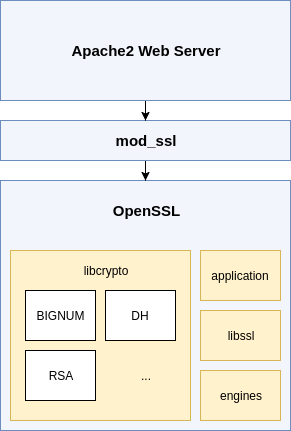
\includegraphics[width=0.4\textwidth]{resources/ch-4/implementation_arch.png}
  \caption{Arsitektur OpenSSL}
  \label{fig:openssl_arch}
\end{figure}

% Cek lagi jumlahnya
Secara default, jumlah maksimal thread maksimum yang akan digunakan oleh OpenSSL untuk menjalankan komputasi big integer secara paralel akan bergantung pada jumlah core yang terdapat pada lingkungan instalasi. Dalam aplikasi yang membutuhkan komputasi yang tinggi setiap thread akan berjalan secara terus menerus. Dengan demikian jumlah thread maksimum akan sama dengan jumlah aplikasi. Namun, aplikasi juga memiliki pilihan konfigurasi untuk menentukan jumlah thread maksimum yang dapat digunakan.
% \todo{cite disini}

\subsection{Batasan Implementasi}
Implementasi dilakukan pada sistem operasi Ubuntu 64 bit. Karena itu, implementasi library big number hanya berfokus pada openssl dengan yang memiliki konfigurasi makro sebagai berikut:
\begin{enumerate}[label=\roman*.]
  \item BN\_ULONG = unsigned long long
  \item OPENSSL\_SMALL\_FOOTPRINT = false
  \item BN\_MUL\_COMBA = true
  \item BN\_RECURSION = true

\end{enumerate}

Konfigurasi makro tersebut digunakan dalam pemilihan dan manajemen struktur data yang digunakan serta pemilihan algoritma pada bagian tertentu. Sebagai contoh, algoritma yang digunakan dalam perkalian adalah algoritma karatsuba dan algoritma comba pada basis rekursif.

\subsection{Struktur Data Big Integer} \label{sec:bignum_struct}
Pada OpenSSL, sebuah big integer direpresentasikan dalam struktur data BIGNUM. BIGNUM terdiri dari sebuah array dengan ukuran dinamis dan beberapa integer yang menyimpan informasi tambahan. Dengan demikian secara teori BIGNUM tidak memiliki nilai maksimum. Untuk keperluan paralelisasi, BIGNUM dapat digunakan tanpa mengubah strukturnya sedikitpun. BIGNUM sendiri merupakan sebuah \textit{struct} yang memiliki deklarasi sebagai berikut.

\begin{lstlisting}[caption=Struktur Data bignum]
struct bignum_st {
       BN_ULONG *d;
       int top;
       int dmax;
       int neg;
       int flags;
};
\end{lstlisting}

|BN_ULONG| sendiri adalah sebuah makro yang menggantikan |unsigned long| pada komputer 32 bit atau |unsigned long long| pada komputer 64 bit.

|d| adalah pointer untuk array of integer.

|top| merupakan index |d| yang terakhir digunakan plus satu.

|dmax| adalah panjang maksimum array yang telah dibuat. |neg| bernilai satu jika BIGNUM bernilai negatif.

\todo[inline]{jelasin BN\_CTX}

\subsection{Struktur File \textit{Source Code}}

\missingfigure{Struktur file}

Struktur \textit{source code} dapat dilihat pada Gambar XXX. Direktori utama berisi pembagian dari fungsi aplikasi yang ada dalam OpenSSL. Beberapa fungsi tersebut adalah direktori |doc| yang berisi dokumentasi OpenSSL, |crypto| yang berisi library kriptografi, |ssl| yang berisi dari library komunikasi ssl, serta |test| yang berisi unit test yang dimiliki OpenSSL.

Direktori |crypto| berisi modul-modul yang membentuk libcrypto, dengan setiap modul terbentuk dalam sebuah direktori yang berbeda. Modul |bn| merupakan modul yang mengatasi perhitungan operasi aritmatika big integer. Selain itu, modul |dh| dan |rsa| merupakan modul yang menangani komputasi Diffie-Hellman dan RSA pada OpenSSL.

Modul |bn| memiliki beberapa submodul masing-masing merupakan file yang berbeda. Setiap submodul sendiri mengatasi fungsi yang terkait dengan submodul tersebut, ataupun operasi yang komputasinya mirip dengan submodul. Sebagai contoh, submodul |bn_add| merupakan submodul yang mengatasi operasi penjumlahan dan pengurangan pada big integer. Selain itu, submodul |bn_mul| merupakan submodul yang mengatasi operasi perkalian serta pemilihan algoritma perkalian yang digunakan dalam OpenSSL.

\subsection{Modul Operasi Aritmatika}
\subsubsection{Submodul Penjumlahan dan Pengurangan}
Modul penjumlahan dan pengurangan terdapat pada file BN\_add.c. Fungsi BN\_add() pada modul ini melakukan pengolahan data pada a dan b seperti mengecek negatif dan mengecek panjang masing-masing array. Hasil pengecekan tersebut akan digunakan untuk melakukan operasi lebih lanjut. Jika a dan b memiliki tanda yang berbeda, akan dipanggil fungsi BN\_usub() selain itu akan dipanggil fungsi BN\_uadd(). BN\_uadd() dan BN\_usub() melakukan pengolahan data pada a dan b sehingga terdapat representasi array yang dapat diolah oleh BN\_add\_words() dan BN\_sub\_words(). Daftar fungsi yang terdapat pada submodul penjumlahan dan pengurangan dapat dilihat pada Tabel \ref{tab:bn_add_func}.

BN\_add\_words merupakan fungsi yang menerima masukan dua array dengan ukuran yang sama dan menjumlahkannya secara sekuensial. Penerapan algoritma \ref{alg:add} pada OpenSSL terdapat pada fungsi ini.

\begin{table}[!h]
  \caption{Fungsi dalam submodul bn\_add}
  \label{tab:bn_add_func}
  \begin{tabular}{R{2.5cm}L{10.5cm}}
\toprule
\textbf{Header Fungsi} & |int BN_add(BIGNUM *r, const BIGNUM *a, const BIGNUM *b)|    \\ \midrule
\textit{Deskripsi}    & Menjumlahkan a dan b dan menyimpan hasilnya pada r $(a+b=r)$ \\
\textit{Prekondisi}    & - \\
\textit{Return Value}  & 1 jika fungsi berhasil dilakukan dan 0 jika tidak
 \\ \bottomrule
\textbf{Header Fungsi} & |int BN_sub(BIGNUM *r, const BIGNUM *a, const BIGNUM *b)|    \\ \midrule
\textit{Deskripsi}    & Mengurangi b dari a dan menyimpan hasilnya pada r $(a-b=r)$ \\
\textit{Prekondisi}    & - \\
\textit{Return Value}  & 1 jika fungsi berhasil dilakukan dan 0 jika tidak
 \\ \bottomrule
\textbf{Header Fungsi} & |int BN_uadd(BIGNUM *r, const BIGNUM *a, const BIGNUM *b)|    \\ \midrule
\textit{Deskripsi}    & Menjumlahkan a dan b dan menyimpan hasilnya pada r $(a+b=r)$ \\
\textit{Prekondisi}    & $a \geq 0$,$ b \geq 0$ \\
\textit{Return Value}  & 1 jika fungsi berhasil dilakukan dan 0 jika tidak
 \\ \bottomrule
\textbf{Header Fungsi} & |int BN_usub(BIGNUM *r, const BIGNUM *a, const BIGNUM *b)|    \\ \midrule
\textit{Deskripsi}    & Mengurangi b dari a dan menyimpan hasilnya pada r $(a-b=r)$ \\
\textit{Prekondisi}    & $a \geq 0$, $b \geq 0$, $a \geq b$ \\
\textit{Return Value}  & 1 jika fungsi berhasil dilakukan dan 0 jika tidak
 \\ \bottomrule
\end{tabular}

\end{table}

\subsubsection{Modul Perkalian}
\begin{table}[h]
  \caption{Fungsi dalam submodul bn\_add}
  \begin{tabular}{R{2.5cm}L{10.5cm}}
\toprule
\textbf{Header Fungsi} & |int BN_mul(BIGNUM *r, const BIGNUM *a, const BIGNUM *b, BN_CTX *ctx)|    \\ \midrule
\textit{Deskripsi}     & Mengalikan $b$ pada $a$ dan menyimpan hasilya dalam $r, (r = a * b)$. \\
\textit{Prekondisi}    & - \\
\textit{Return Value}  & 1 jika fungsi berhasil dilakukan dan 0 jika tidak
 \\ \bottomrule
\textbf{Header Fungsi} & |void bn_mul_normal(BN_ULONG *r, BN_ULONG *a, int na, BN_ULONG *b, int nb)|    \\ \midrule
\textit{Deskripsi}     &  Perkalian $a$ dan $b$ dengan menggunakan algoritma perkalian panjang, dengan $na$ adalah panjang $a$ dan $nb$ adalah panjang $b$.\\
\textit{Prekondisi}    &  -\\
\textit{Return Value}  & 1 jika fungsi berhasil dilakukan dan 0 jika tidak
 \\ \bottomrule
\textbf{Header Fungsi} & |void bn_mul_recursive(BN_ULONG *r, BN_ULONG *a, BN_ULONG *b, int n2 int dna, int dnb, BN_ULONG *t)|    \\ \midrule
\textit{Deskripsi}     &  Perkalian $a$ dan $b$ dengan menggunakan algoritma perkalian karatsuba. $n2$ adalah panjang hasil perkalian, dengan $dna = length(a) - n2$ dan $dnb = length(b) - n2$\\
\textit{Prekondisi}    & $length(r) = 2*n2$. $ length(t) = 2*n2$. $n2 = 2^k, k \in \mathbb{Z}. $\\
\textit{Return Value}  & 1 jika fungsi berhasil dilakukan dan 0 jika tidak
 \\ \bottomrule
\end{tabular}

\end{table}

\subsubsection{Submodul Pembagian}
\begin{table}[h]
  \caption{Fungsi dalam submodul bn\_add}
  \begin{tabular}{R{2.5cm}L{10.5cm}}
\toprule
\textbf{Header Fungsi} & |BN_div(BIGNUM *dv, BIGNUM *rm, const BIGNUM *num, const BIGNUM *divisor, BN_CTX *ctx)|    \\ \midrule
\textit{Deskripsi}     &  Membagi num dengan divisor, hasil pembagian disimpan sebagai dv dan sisa pembagian disimpan sebagai rm. Baik div maupun rm bisa menjadi NULL jika hasil atau sisa pembagian tidak dibutuhkan. \\
\textit{Prekondisi}    &  -\\
\textit{Return Value}  &1 jika fungsi berhasil dilakukan dan 0 jika tidak
 \\ \bottomrule
\textbf{Header Fungsi} & |int bn_left_align(BIGNUM *num)|    \\ \midrule
\textit{Deskripsi}     &  Normalisasi BIGNUM $num$ agar $num > \beta/2$\\
\textit{Prekondisi}    & - \\
\textit{Return Value}  & 1 jika fungsi berhasil dilakukan dan 0 jika tidak
 \\ \bottomrule
\end{tabular}

\end{table}

\subsubsection{Submodul Asm}
\begin{table}[h]
  \caption{Fungsi dalam submodul bn\_add}
  \begin{tabular}{R{2.5cm}L{10.5cm}}
\toprule
\textbf{Header Fungsi} & |BN_ULONG bn_add_words(BN_ULONG *a, const BN_ULONG *a, const BN_ULONG *b, int n)|    \\ \midrule
\textit{Deskripsi}     &   \\
\textit{Prekondisi}    &  -\\
\textit{Return Value}  &
 \\ \bottomrule
\textbf{Header Fungsi} & |BN_ULONG bn_sub_words(BN_ULONG *r, const BN_ULONG *a, const BN_ULONG *b, int n)|    \\ \midrule
\textit{Deskripsi}     &   \\
\textit{Prekondisi}    &  -\\
\textit{Return Value}  &
 \\ \bottomrule
\textbf{Header Fungsi} & |BN_ULONG bn_mul_words(BN_ULONG *rp, const BN_ULONG *ap, int num, BN_ULONG w)|    \\ \midrule
\textit{Deskripsi}     &   \\
\textit{Prekondisi}    &  -\\
\textit{Return Value}  &
 \\ \bottomrule
\textbf{Header Fungsi} & |BN_ULONG bn_mul_add_words(BN_ULONG *rp, const BN_ULONG *ap, int num, BN_ULONG w)|    \\ \midrule
\textit{Deskripsi}     &   \\
\textit{Prekondisi}    &  -\\
\textit{Return Value}  &
 \\ \bottomrule
\textbf{Header Fungsi} & |BN_ULONG bn_div_words(BN_ULONG h, BN_ULONG l, BN_ULONG d)|    \\ \midrule
\textit{Deskripsi}     &   \\
\textit{Prekondisi}    &  -\\
\textit{Return Value}  &
 \\ \bottomrule
\end{tabular}

\end{table}

  
\section{Evaluasi}
\subsection{Lingkungan Pengujian}
4 digitalocean cpu based, 1 openssl basic 1 core, 1core, 16core, 32core. Semua pake OS, apache versi yang sama
\missingfigure{arsitektur lingkungan pengujian}
\subsection{Skenario Pengujian}
Install apache, test pake apachebench, get waktu, rata2 tiga kali
\subsection{Hasil dan Analisis}
\subsubsection{Hasil Pengujian}
  Langsung data speedup aja, data raw simpen di lampiran

  \begin{table}[ht]
  \caption{Test table} % title of Table
  \centering % used for centering table
  \begin{tabular}{c c c c} % centered columns (4 columns)
  \hline\hline %inserts double horizontal lines
  Case & Method\#1 & Method\#2 & Method\#3 \\ [0.5ex] % inserts table
  %heading
  \hline % inserts single horizontal line
  1 & 50 & 837 & 970 \\ % inserting body of the table
  2 & 47 & 877 & 230 \\
  3 & 31 & 25 & 415 \\
  4 & 35 & 144 & 2356 \\
  5 & 45 & 300 & 556 \\ [1ex] % [1ex] adds vertical space
  \hline %inserts single line
  \end{tabular}
  \label{table:nonlin} % is used to refer this table in the text
  \end{table}

\subsubsection{Analisis Pengujian}


    %!TEX root = ../../tugas-akhir.tex
\chapter{PENUTUP}

  \section{Kesimpulan}
    % \blindtext

  \section{Saran}
    % \blindtext


    % -------------------------------------------------------------------------%
    % Daftar Pustaka
    % -------------------------------------------------------------------------%
    \renewcommand{\bibname}{Daftar Pustaka}
    \cleardoublepage
    \phantomsection
    \addcontentsline{toc}{chapter}{DAFTAR PUSTAKA}
    \bibliography{references}


    %-------------------------------------------------------------------------%
    % Lampiran
    %-------------------------------------------------------------------------%
    \titleformat{\chapter}[block]
      {\normalsize\bfseries}
      {\chaptertitlename\ \thechapter}{0pt}
        {\normalsize\bfseries}
    \titlespacing*{\chapter}{0pt}{-25pt}{20pt}

    \setcounter{chapter}{0}

    % \addtocontents{toc}{\protect\setcounter{tocdepth}{-2}}

    % \setcounter{secnumdepth}{-2}
    % \begin{appendices}
    \renewcommand{\chaptername}{Lampiran}
    \renewcommand{\thechapter}{\Alph{chapter}. }
    
    \appendix{Daftar Fungsi dalam Modul bn yang Berkaitan dengan Operasi Aritmatika}\label{sec:bn_func_all}

Berikut adalah fungsi yang merupakan operasi aritmatika dalam modul big integer.

\VerbatimInput[label=\fbox{list-func.txt}]{resources/text/bn_func_all.txt}

    \chapter{Pemanggilan Library Big Number} \label{bn_func_call}
\todo{Benerin nomor lampiran}
Berikut adalah hasil menjalankan \textit{grep} dengan pattern fungsi-fungsi Big Number pada modul Diffie Hellman dan RSA pada OpenSSL.

\paragraph{Diffie Hellman}
Modul Diffie Hellman pada OpenSSL terdapat pada direktori |openssl/crypto/dh|

\VerbatimInput[label=\fbox{dh.txt}]{resources/bn_grep/grep_result_dh.txt}

\paragraph{RSA}
Modul RSA pada OpenSSL terdapat pada direktori |openssl/crypto/rsa|

\VerbatimInput[label=\fbox{rsa.txt}]{resources/bn_grep/grep_result_rsa.txt}

    %!TEX root = ../../tugas-akhir.tex

\chapter{Kasus Uji Fungsional} \label{sec:functional_testcase}

Berikut adalah contoh kasus uji yang digunakan dalam pengujian fungsional modul bn dalam OpenSSL. Test uji yang sebenarnya digunakan tidak dimasukkan pada bagian ini karena jumlahnya terlalu banyak.

\paragraph{Penjumlahan dan Pengurangan}
\VerbatimInput[label=\fbox{bn\_sum.txt}]{resources/text/bn_testcase/bn_sum.txt}

\paragraph{Perkalian}
\VerbatimInput[label=\fbox{bn\_mul.txt}]{resources/text/bn_testcase/bn_mul.txt}

\paragraph{Pembagian}
\VerbatimInput[label=\fbox{bn\_div.txt}]{resources/text/bn_testcase/bn_div.txt}

\paragraph{Perpangkatan}
\VerbatimInput[label=\fbox{bn\_exp.txt}]{resources/text/bn_testcase/bn_exp.txt}
%
\paragraph{Perkalian Modular}
\VerbatimInput[label=\fbox{bn\_modmul.txt}]{resources/text/bn_testcase/bn_modmul.txt}
%
\paragraph{Perpangkatan Modular}
\VerbatimInput[label=\fbox{bn\_modexp.txt}]{resources/text/bn_testcase/bn_modexp.txt}


    % \end{appendices}

\end{document}
